% We use the reactive synthesis tool \texttt{Slugs}~\cite{EhlersR16} to compute the shields using the procedure described in Section~\ref{sec:distshield}.
% All experiments were  performed on an Intel i5-5300U 2.30 GHz CPU with 8 GB of RAM.
% \subsection{Shield synthesis comparison}
% We first compare the decentralized synthesis procedure presented in this paper with a centralized synthesis procedure detailed in \cite{multiagentshield}. In a centralized setting, the synthesis time grows exponentially with the number of vertihubs present and the number of vehicles used in the experiment.

% In each sector the safety specification $\varphi_i$ is to not exceed an upper bound of vehicles in each sector. For simplicity, we use the same contract values $\mathcal C_{\shield_j}^{\shield_i} = (A_{\shield_j}^{\shield_i},B_{\shield_j}^{\shield_i})$ referred to as $C$ in Table~\ref{tab:censynth} and maximum vehicle upper bound for the referred to as $N$ for all sectors, though, in principle, this is not necessary. 

% Again, we use the same $N$ for each sector. We compare the two procedures for increasing numbers of sectors in Table.~\ref{tab:censynth}. We report synthesis times for computing the permissive strategy, along with the time for computing the cost-optimal strategy from the permissive strategy. We use a cost function that assigns a cost whenever the shield moves an idle vehicle out of its region in order to disincentivize shields from moving vehicles when it is not required. 
\begin{figure}
    % \hfill 
    \centering
    \scalebox{0.75}{

\definecolor{bodyyel}{HTML}{FFE58F}
\definecolor{bodybl}{HTML}{85A1DC}

    \begin{tikzpicture}[scale=1.0]
		  %  \tikzstyle{system} = [thick,draw=blue,circle,fill=bodybl]
		  %  \tikzstyle{shield} = [thick,draw=red,and gate US,fill=red!20!white]
    %         \tikzstyle{vert} = [thick,draw=blue,rectangle,fill=bodybl,rounded corners]
		  %  \tikzstyle{hub} = [thick,draw=red,and gate US,fill=red!20!white]
            \node[vert](vert1){$\shield^1_1$};
            \node[vert,below=5mm of vert1](vert2){$\shield^1_2$};
            \node[vert,below=5mm of vert2](vert3){$\shield^2_1$};
            
            \node[hub,right=30mm of vert1] (hub1){$\design_1$};
            \node[hub,right=30mm of vert3] (hub2){$\design_2$};
            
            \node[left=10mm of vert1.210,draw=none,text width=1.6cm] (in1) {};
            \node[left=10mm of vert2.210,text width=1.5cm,rectangle,rounded corners,draw,minimum height=50mm,fill=yellow!20!white] (in2) {Orig-Dest requests};
            \node[left=10mm of vert3.145,draw=none,text width=1.6cm] (in3) {};

            \path[name path=odest] (in1)--node[above] {} (vert1.205);
            
            \path[->,draw,very thick] (in2)--node[above] {} (vert2.205);
            \path[->,draw,very thick] (in3)--node[above] {} (vert3.145);
            
            \coordinate[right=2.5mm of vert1.30](c1);
            \coordinate[right=5mm of vert1.330](c2);
            
            \path[draw,very thick] (vert1.30) |- (c1);
            \path[name path=avail1] (vert1.330) |- (c2);
            \path[name path=request2,very thick, draw] (vert2.30) -| (c1);
            \path[draw,very thick] (vert2.330) -| (c2);
            
            \path[name intersections={of=avail1 and request2}];
            \coordinate (S) at (intersection-1);
            \path[name path=circle] (S) circle(1.0mm);
            \path[name intersections={of = circle and avail1}];
            \coordinate (I1) at (intersection-1);
            \coordinate (I2) at (intersection-2);
            \path[draw,very thick] (vert1.330) -- (I2);
            \path[draw,very thick] (I1) -- (c2);
            \tkzDrawArc[color=black,very thick](S,I1)(I2);
            
            
            \path[->,draw,very thick] (c1) -- node[above]{Requests} (hub1.150);
            \path[->,draw,very thick] (c2) -- node[below]{Availability} (hub1.210);
            
            \coordinate[above right=10mm and 5mm of hub1.30](out1);
            \coordinate[below right=10mm and 5mm of hub2.330](out2);
            \path[draw,very thick] (hub1.30) -| (out1);
            \path[draw,very thick] (hub2.330) -| (out2);
            \path[->,draw,very thick] (vert3.30) -- node[above]{Requests} (hub2.150);
            \path[->,draw,very thick] (vert3.330) -- node[below]{Availability}  (hub2.210);
            

            \coordinate[right=12.5mm of hub1.0] (loiter1);
            \coordinate[right=12.5mm of hub2.0] (loiter2);
             \node [below left=15mm and 0mm of loiter2] {$V$};
            \coordinate[above left=10mm and 5mm of vert1.150] (X1);
            \coordinate[below left=10mm and 5mm of vert3.210] (X2);
            \coordinate[below right=12.5mm and 2.5mm of hub1.330](Y1);
            \coordinate[above right=12.5mm and 5.0mm of hub2.30](Y2);
            
            \path[->,draw, very thick] (hub1.0) --node[above right]{Loiter} (loiter1);
            \path[->,draw, very thick] (hub2.0) --node[above right]{Loiter} (loiter2);
            \path[draw, very thick] (out1) -- node[above]{Land allocation} (X1);
            \path[draw, very thick] (out2) -- node[below]{Land allocation} (X2);
            \path[->,draw,very thick](X1) |- (vert1.150);
            \path[->,draw,very thick,name path=land2](X1) |- (vert2.150);
            \path[->,draw,very thick](X2) |- (vert3.210);
            
            \path[draw,very thick] (hub1.330) -| node[below right] {Pass} (Y1);
            \path[draw,very thick] (hub2.30) -| node[above right=5mm and 0mm] {Pass} (Y2);
            \path[->,draw,very thick] (Y1) -| (hub2.120);
            \path[->,draw,very thick] (Y2) -| (hub1.240);
            
            \path[name intersections={of=odest and land2}];
            \coordinate (S2) at (intersection-1);
            \path[name path=circle2] (S2) circle(1.0mm);
            \path[name intersections={of = circle2 and odest}];
            \coordinate (I1) at (intersection-1);
            \coordinate (I2) at (intersection-2);
            \path[draw,very thick] (in1) -- (I2);
            \path[draw,very thick] (I1) -- (vert1.205);
            \tkzDrawArc[color=black,very thick](S2,I1)(I2);
            
            % \begin{scope}[on background layer]
        \node [below right=-42.5mm and -13.0mm of vert3,text width=55mm,draw,dashed,minimum height=60mm] (box) {};
       
            % \end{scope}

            
            
            
            
            
            % \node[system,above right=5mm and 25mm of mdp] (D1) {$\design_1$};
            % \node[system,right= 24mm of mdp] (D2) {$\design_2$};
            % \node[system,below right=5mm and 25mm of mdp] (D3) {$\design_3$};
            % \node[shield,right=15mm of D1] (S1) {$\shield_1$};
            % \node[shield,right=15mm of D2] (S2) {$\shield_2$};
            % \node[shield,right=15mm of D3] (S3) {$\shield_3$};
            % \coordinate[right=15mm of mdp] (X);
            % \node[right=10mm of S1] (X1){};
            % \node[right=10mm of S2] (X2){};
            % \node[right=10mm of S3] (X3){};
            % \path[->,draw,thick] (X)--node[above left,near end] {$\ialphabetx{1}$} (D1);
            % \path[->,draw,thick] (X)--node[above] {$\ialphabetx{2}$} (D2);
            % \path[->,draw,thick] (X)--node[below left,near end] {$\ialphabetx{3}$} (D3);
            % \path[->,draw,thick] (D1)--node[above] {$\oalphabetx{1}$} (S1);
            % \path[->,draw,thick] (D2)--node[above] {$\oalphabetx{2}$} (S2);
            % \path[->,draw,thick] (D3)--node[below] {$\oalphabetx{3}$} (S3);
            % \path[->,draw,thick] (D3)--node[at end,below right] {$\oalphabetx{3}$} (S2);
            % \path[->,draw,thick] (D2)--node[at end,above right] {$\oalphabetx{2}$} (S3);
            % \path[->,draw,thick] (D2)--node[below right,at end] {$\oalphabetx{2}$} (S1);
            % \path[->,draw,thick] (D1)--node[above right,at end] {$\oalphabetx{1}$} (S2);
            % \path[->,draw,thick] (S1)--node[above] {$\oalphabetx{1}'$} (X1);
            % \path[->,draw,thick] (S2)--node[above] {$\oalphabetx{2}'$} (X2);
            % \path[->,draw,thick] (S3)--node[above] {$\oalphabetx{3}'$} (X3);
            
                        
		\end{tikzpicture}

}
        \caption{Implementation of the architecture in Figure~\ref{fig:dist_shield} for UAM ATM case study. }
	    \label{fig:exp_shield}
    \end{figure}



% \begin{table}[]
% \caption{Synthesis time comparison between centralized and localized methods.}\label{tab:censynth}
% \begin{tabular}{lllllll}
% \toprule
%  & Sectors & $N$ & $C$ & Perm. strategy time (s) & Opt. strategy time (s) &  \\
% \midrule
% \multicolumn{1}{c}{\multirow{4}{*}{\textbf{Centralized}}} & 3 & 2 & 2 & 43 & 17 &  \\
% \multicolumn{1}{c}{} & 5 & 3 & 3 & 1840 & 1489 &  \\
% \multicolumn{1}{c}{} & 7 & 4 & 4 & Time out & Time out &  \\
% \multicolumn{1}{c}{} & 9 & 5 & 5 & Time out & Time out &  \\ \hline
% \multirow{4}{*}{\textbf{Localized}} & 3 & 2 & 2 & 13 & 10 &  \\
%  & 5 & 3 & 3 & 123 & 32 &  \\
%  & 7 & 4 & 4 & 219 & 111 &  \\
%  & 9 & 5 & 5 & 470 & 286 & \\
%  \bottomrule
% \end{tabular}
% \end{table}

%Note that the decentralized synthesis procedure significantly outperforms the synthesis time of the centralized case. In the last two trials, the centralized shield synthesis timed out unsuccessfully.

\subsection{Simulation setting}
We demonstrate our approach on large-volume UAM air traffic data. The data used in the simulation was generated by NASA Langley in conjunction with partners performing UAM demand studies, and is in a format compatible with the Mission Planner Algorithm~\cite{guerreiro2019mission} developed at NASA Langley. The data contains simulated, timestamped on-demand requests for origin-destination trips. The dataset includes the position of 1000 vertiports which serve as the origin-destination pairs. 
\textcolor{black}{In practice, the vertihub placement and size will correspond to physical infrastructure and we thus treat them as given inputs to the controller synthesis problem. 
%While these decisions are beyond the scope of the paper, for this case study we perform the arbitrary task of selecting the vertihubs' centroids by using k-means clustering on the dataset vertiport locations.
}  
Requests are spawned when the timestamp corresponding to a trip request in the data is reached. Each vertihub handles the requests of the UAM vehicles as they come into range (defined by the circles in Fig.~\ref{fig:sim}). \textcolor{black}{Note that increasing the number of vertihubs leads to the balkanization of the airspace.}

Each vehicle has a process flow from take-off to landing (Fig.~\ref{fig:aircraftprocess}).
As a vehicle enters the range of a vertihub, it sends the vertihub controller a request to either land or pass through.
Then the vertihub controller sends one of three commands:
\begin{enumerate}
    \item If permission is granted to pass-through, the vehicle (green) flies to the next vertihub and requests access.
    \item If permission is granted to land, the vehicle (yellow) approaches the requested vertiport and sends a landing request to the vertiport controller.
    \item If neither permission is granted, the vehicle loiters (orange) and repeats its request.
 
\end{enumerate}

\begin{figure}
    \centering
    \scalebox{0.75}{\definecolor{bg}{HTML}{ddeedd}
\definecolor{comp}{HTML}{c2d4dd}
\definecolor{impl}{HTML}{b0aac0}
\definecolor{ligb}{HTML}{5E7FC6}
\definecolor{bodybl}{HTML}{85A1DC}
\definecolor{headbl}{HTML}{264C9C}
\definecolor{bgyel}{HTML}{FFDC6B}
\definecolor{bodyyel}{HTML}{FFE58F}
\definecolor{headyel}{HTML}{E9BB25}
\definecolor{gr1}{HTML}{00FF00}
\definecolor{or1}{HTML}{FFAA00}
\definecolor{ye1}{HTML}{FFFF00}

% Define block styles
\tikzstyle{decision} = [diamond, draw, fill=blue!20, 
text width=4.5em, text badly centered, node distance=3cm, inner sep=0pt]
\tikzstyle{block} = [rectangle, draw, fill=blue!20, 
text width=5em, text centered, rounded corners, minimum height=4em]
\tikzstyle{line} = [draw, -latex']
\tikzstyle{cloud} = [draw, ellipse,fill=red!20, node distance=3cm,
minimum height=2em]
\def\checkmark{\tikz\fill[scale=0.6](0,.35) -- (.25,0) -- (1,.7) -- (.25,.15) -- cycle;} 
%
\centering
\begin{tikzpicture}[every node/.style={draw, text centered, shape=rectangle, rounded corners, text width=3cm, minimum height=0.8cm, inner sep=5pt}]
%\tikzstyle{outer}= [draw, text centered, shape=rectangle, text width=2cm, minimum height=1cm]
%\tikzstyle{inner}=[draw, text centered, shape=rectangle, rounded corners, text width=3.8cm, minimum height=1.1cm, inner sep=5pt]
\tikzstyle{decision} = [diamond, draw, aspect=3 , inner sep=3pt]


\node[fill=gr1!20!white] (launch){Launch};
\node[below=0.5cm of launch,fill=gr1!20!white] (move) {Flight};
\node[fill=blue!10!white,decision,below=0.5cm of move] (range) {Within range?};
\node[below=0.5cm of range,fill=or1!20!white] (loiter) {Loiter};
\node[fill=blue!10!white,decision,below=0.5cm of loiter] (assign) {Assigned?};
\node[below=0.5cm of assign,fill=ye1!20!white] (approach) {Approach};
\node[right=0.5cm of approach,fill=red!20!white,text width=1.5cm,inner sep=1pt] (land) {Land};

\path [line,-latex',very thick] (launch.south) -- (move.north);
\path [line,-latex',very thick] (move.south) -- (range.north);
\path [line,-latex', very thick] (range.south) --node[draw=none,right=-1.2cm]{Yes} (loiter.north);
\path [line,-latex', very thick] (range.east) -- node[draw=none,above=1pt] {No} ++(1.0,0)   |- (move.east);
\path [line,-latex', very thick] (loiter.south) --node[draw=none,left=-1cm]{Request} (assign.north);
\path [line,-latex', very thick] (assign.south) --node[draw=none,right=-1.2cm]{Land} (approach.north);
\path [line,-latex', very thick] (assign.east)  -- node[draw=none,above=1pt] {No} ++(1.0,0) |- (loiter.east);
\path [line,-latex', very thick] (assign.west)  -- node[draw=none,below=1pt] {Pass-through} ++(-1.0,0) |- (move.west);
\path [line,-latex', very thick] (approach.east) -- (land.west);


\end{tikzpicture}}
    \caption{Process flow for an individual vehicle - during flight it checks whether it is in range of a vertihub. Once within range, the vehicle loiters and creates a request to either land or pass-through. The colors in the figure are used in the simulations to represent the current status of the vehicle.}
    \label{fig:aircraftprocess}
\end{figure}




% \begin{figure}[h!]
%     \centering
%     \newcommand{\OperatorSpaceA}[3]{
				%\draw[rounded corners = 15pt,dashed] (#1-#4,#2-#5) rectangle (#1+#4,#2+#5);
		\fill[fill=green,opacity=0.2] (#1,#2) circle (#3);
		\draw[draw = black,dashed](#1,#2) circle (#3);
		%\node at (#1,#2-#5+0.5) {$V_{#6}$};
	}

	
	
\begin{tikzpicture}[scale=0.8]
	\OperatorSpaceA{0}{0}{1}
	\node at (-0.5,0.5){$V_1$};
	\OperatorSpaceA{1}{1}{1}
	\node at (0.5,1.5){$V_2$};
	\OperatorSpaceA{1}{2.8}{1}
	\node at (0.5,3.0){$V_3$};
	\OperatorSpaceA{2}{2}{1}
	\node at (1.85,1.85){$V_4$};
	\OperatorSpaceA{1.3}{-0.2}{1}
	\node at (1.5,-0.5){$V_5$};
	\OperatorSpaceA{4}{3}{1}
	\node at (4.5,3){$V_6$};
	\OperatorSpaceA{2.8}{3.4}{1}
	\node at (3.75,4.35){$V_7$};
	\OperatorSpaceA{3.1}{1.8}{1}
	\node at (3.3,1.3){$V_8$};
	\OperatorSpaceA{2}{4}{1}
	\node at (2,4.65){$V_9$};
	%\node at (10+5.25,-6.5){$S_5$};
	\fill[blue] (-0.5,-0.5) rectangle (-0.25,-0.25);
	\fill[black] (1.5,3.75) rectangle (1.75,4.0);
	\fill[black] (2.0,4.0) rectangle (2.25,4.25);
	\fill[magenta] (2.5,4.0) rectangle (2.75,4.25);
	\fill[red] (3.5,1.75) rectangle (3.75,2.00);
    \draw (1.7,-0.2) node[cross,red]{};
    \draw (4.05,3) node[cross,blue]{};
    \draw (3.25,1.75) node[cross,magenta]{};
	%\node at (15-4.25,5+3.25){$S_6$};
% 	\draw (17,5) node[cross,blue]{};
% 	\draw[blue,line width = 0.5mm] plot [smooth,tension=1] coordinates{(-1.5,-1.5) (3,0.5) (10,0) (17,5)};
% 	\draw (-0.5,2) node[cross,black]{};
% 	\fill[black] (7.5,-5.5) rectangle (7.0,-5.0);
% 	\draw[black,line width = 0.5mm] plot [smooth,tension=1] coordinates{(-0.5,2) (3,-0.5) (7,-5.0)};
	
\end{tikzpicture}
%     \caption{Example UAM environment with 9 regions ($V_1,\cdots,V_9$), 5 UAM vehicles and 3 destinations. The initial locations and desired destinations of $\Agent_1$ (blue), $\Agent_2$ (red) and $\Agent_3$ (magenta) are given by the squares and crosses respectively. Agents $\Agent_4$ and $\Agent_5$ (black squares) are initially loitering in sector $V_9$ with no task requirement. }
%     \label{fig:env}
% \end{figure}
% \begin{figure}
%     \centering
%     % \includegraphics[width=0.48\textwidth]{pics/ports.eps}
%     \label{fig:my_label}
% \end{figure}




%\subsection{Simulation Setting}
\label{ssec:SimSet}
% \textcolor{green}{When we describe interacting vertihubs, we refer to the segments where their regions of control overlap, see Fig.~\ref{fig:sim} for an example of an environment with sparse overlapping. Note that only the number of overlapping regions rather than the physical area of the overlapping regions is consequential to the aircraft's implemented behavior its process flow in Fig.~\ref{fig:aircraftprocess}.}
\textcolor{black}{In order to demonstrate the qualitative behavior of the global system, we examine the procedure with multiple operating vertihubs in three different settings where the vehicles are operating in: 
(i) an airspace covered by vertihubs that have many overlapping regions -- the many intersecting regions of control require a vehicle to receive many permissions to complete its mission.
(ii) \emph{sparsely interacting} vertihubs -- an airspace with only a few overlapping regions of control. Vehicles passing through these vertihubs negotiate few permissions.
 (iii) \emph{closely linked} vertihubs -- a special condition where the overall airspace has few overlapping regions of control but the overlapping regions are physically close together. In this scenario, the vehicles' missions compel them to pass through these regions simulating congestion a potential bottleneck. 
 } 

All vertihub controllers must satisfy the following specifications: (1) landing or pass-through requests must be approved in less than $T$ steps and (2) there can be no more than $N$ vehicles in the region of the vertihub. 
All vertiport controllers must satisfy the following: no more than $M$ vehicles can land at any given time. The landing time is treated as an environment input and can vary based on the vehicle and weather conditions. The contract between the vertiport and vertihub states that a vertiport may not allow a vehicle to take off for up to $L$ steps and must clear a landing spot in at most $K$ steps. The vertihub controllers have contracts with connected controllers agreeing to let vehicles loiter in their regions for $t < T$ timesteps. These contracts allow vertihub controllers to land or let vehicles pass through while incoming vehicles loiter in neighboring regions.
The resulting video simulations for each setting can be seen in  \href{https://u-t-autonomous.github.io/Decentralized-UAM-Traffic-Management/}{https://u-t-autonomous.github.io/Decentralized-UAM-Traffic-Management/}.
\textcolor{black}{Also included in the link are further comparisons with different physical architectures for vertihub placement - in particular we compare scenario (i) when the airspace is covered by double the number of the vertihubs. The average loiter time for vehicles in setting (i) was approximately 3\% less per vehicle for the environment with more vertihubs, however, we note that this is not true in general and will depend on the specific network topology and specifications.}
%\textcolor{green}{Note that quantitative analysis and optimizing for minimum loiter times are of interest to this problem but the controllers operating in these case studies are only concerned with correctness}
\begin{figure}
    \centering
    % \subfloat[Set of VTOL pads]{\includegraphics[trim={16cm 0cm 10cm 0cm},clip,width=0.48\textwidth,height=0.48\textwidth]{pics/ports.eps}}\\
    \subfloat[]{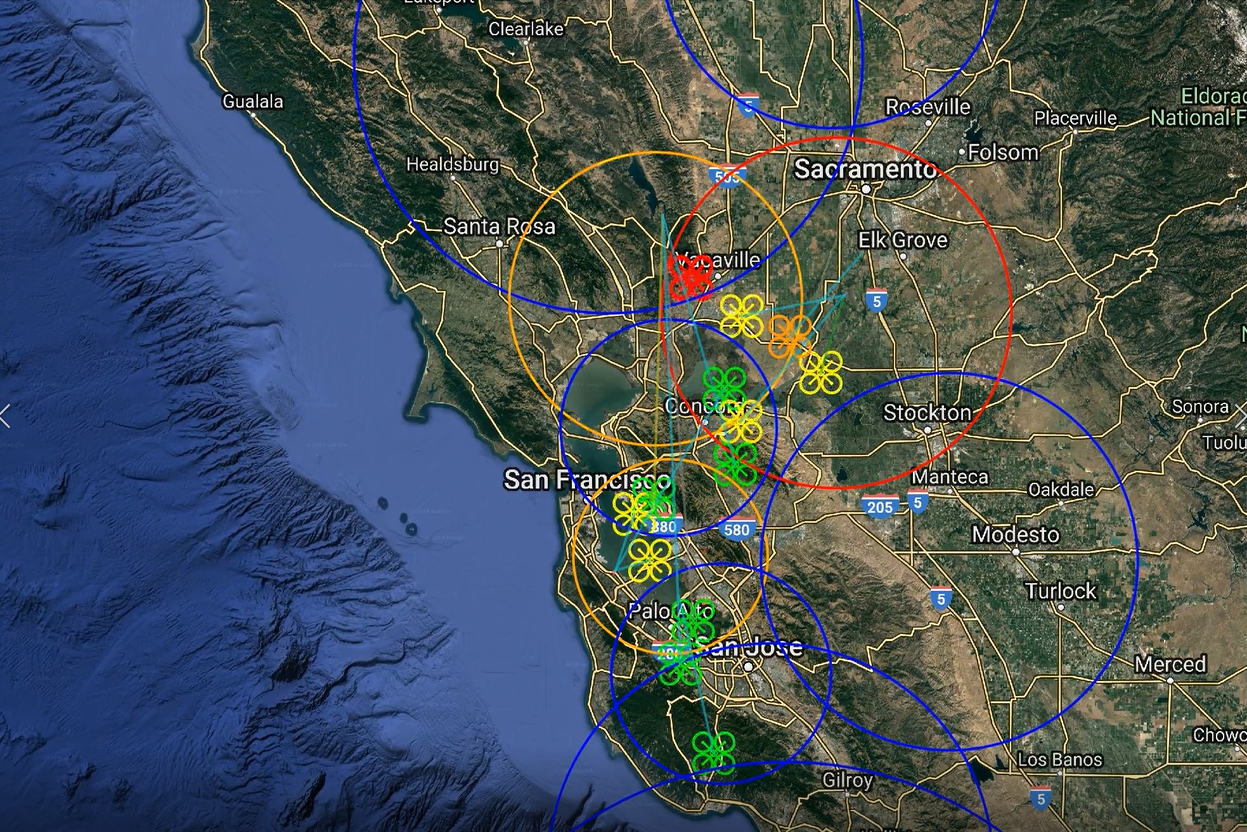
\includegraphics[trim={5cm 3cm 3cm 2.75cm},clip,width=0.42\textwidth]{UAM-TCNS/Towers.PNG}}
    \caption{
    \textcolor{black}{Screenshot of the simulation environment - Operating regions for each vertihub controller and their ranges are indicated by blue circles.
     Green agents are in flight mode, orange agents are loitering, yellow agents are allocated for landing/passing-through and red agents are those that have landed. If a vertihub controller circle is red, then it will accept no more agents until the agents inside have landed or have been accepted to pass through to another region.
     }
    }
    \label{fig:sim}
\end{figure}

\begin{figure*}[h]
\centering
    \subfloat[Landing \label{fig:land}]{
    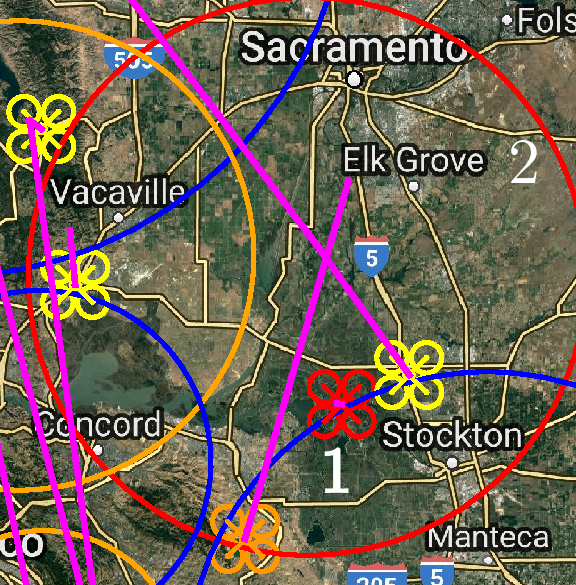
\includegraphics[width=0.25\textwidth]{UAM-TCNS/pics/sequence_100a.png}}~
    \subfloat[Free slot \label{fig:free}]{
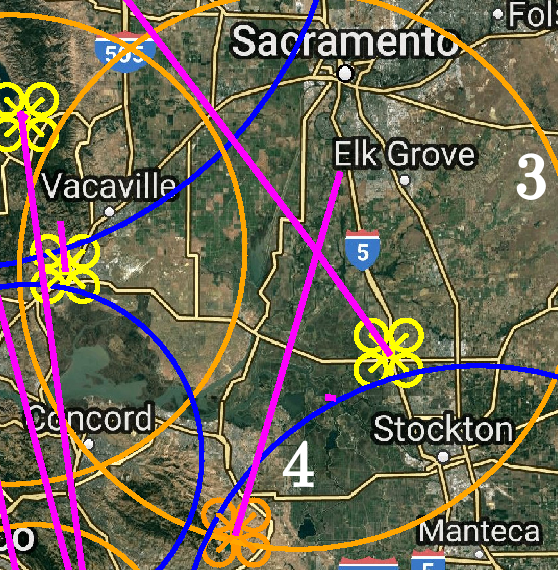
\includegraphics[width=0.25\textwidth]{UAM-TCNS/pics/sequence_103a.png}}~
    \subfloat[Allocated \label{fig:allocate}]{
    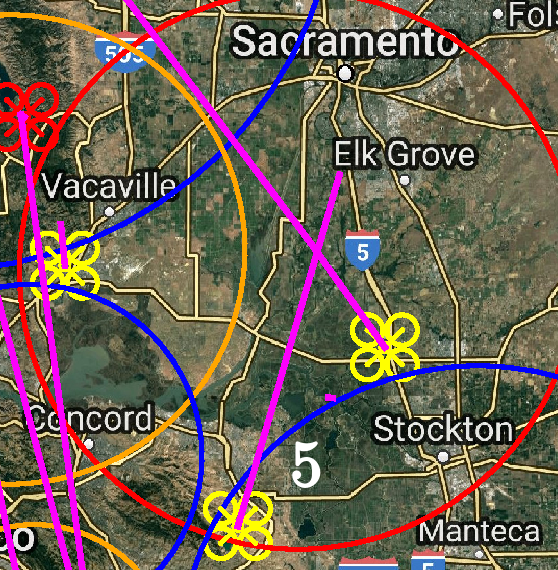
\includegraphics[width=0.25\textwidth]{UAM-TCNS/pics/sequence_104a.png}}
    \caption{\textcolor{black}{Time sequence of a UAV landing ($1$) at a vertiport, which opens up a free slot for the vertihub ($2\rightarrow3$). The hub then allocates another UAV ($4\rightarrow 5$) to land at a free slot in one of the vertiports.}}
    \label{fig:sequence}
\end{figure*}

\subsection{Qualitative Results}

Figure~\ref{fig:sequence} contains an example of the allocation behavior for multiple agents approaching a single vertihub.
\textcolor{black}{Initially the vertihub is informed by the vertiports that there are no slots available for landing (see $2$ in Fig.~\ref{fig:land}). Subsequent to an agent landing ($1$ lands), an additional slot opens (see $3$ in Fig.~\ref{fig:free}).
Finally, the vertihub allocates a slot to a requesting vehicle ($4$ becomes $5$ in figure~\ref{fig:allocate}).} 

For each simulation setting, the vertihub interactions affect how vehicles are allocated and subsequently where they loiter.
In the case of (i), allocation bottlenecks tend to occur upon vehicle launch -- as a vehicle launches it waits for permission to move and thus bottlenecks are limited by the operating number of vehicles in the vertihub.
For (ii), there are significantly fewer bottlenecks but they mostly occur as vehicles either enter or exit a region.
For (iii) we observe the cascading of allocations in each region -- to allocate vehicles in the top region, the vehicles in the middle region must clear and similarly for the middle-lower region interactions.

\subsection{Synthesis time}

We present the synthesis times for the vertihub and vertiport controllers in Table~\ref{tab:hubsyntime}. 
There is an exponential increase in the synthesis time as the number of vertiports in each region is increased.
%Thus, this technique works best when there is not be a large number of vertiports assigned to each vertihub.
The state space of the controllers does not depend on the number of vehicles, allowing us to simulate datasets involving large numbers of vehicles. \textcolor{black}{
The centralized synthesis method in~\cite{bh18} could not be run even in the smallest case as the state space is too large. A decentralized, hierarchical procedure is necessary to handle systems of the necessary size and complexity that UAM will require. Other decentralized techniques such as~\cite{bhnfm} can only handle very restrictive classes of specifications and could not be used to generate controllers in this setting.}

We note that since the synthesis for each vertihub is independent of one another once the contracts are generated, the synthesis procedure for the global system is trivially parallelizable. 



% \begin{table}[htb!]
% 	\centering
% 	\caption{Synthesis times for a vertiport/vertiport controller}
% 	\label{tab:vertsyntime}
% 	\centering
% 	\scalebox{0.9}{
% 		\begin{tabular}{llr}
% 			\toprule
% 		\multicolumn{1}{p{2.5cm}}{} & \multicolumn{1}{p{2.0cm}}{No. of states in controller ($|Q_i^j|$)} &  \multicolumn{1}{p{2.5cm}}{Synthesis time (s)}   \\
% 			\midrule
% 			2 & $6.1\times10^2$ & 0.45      \\
% 			4 & $4.3\times10^4$ & 19.12  \\
% 			8 & $1.9\times10^8$ & 12403.86 \\
% 			\bottomrule
% 	\end{tabular}}
% \end{table}

% \begin{figure}[h!]
% \centering
%     \subfloat[Unshielded: Time = 0 \label{fig:noshieldPolicyA}]{ 	
\begin{tikzpicture}[scale=0.6]
	\OperatorSpaceB{0}{0}{1}
	\node at (-0.5,0.5){$V_1$};
	\OperatorSpaceB{1}{1}{1}
	\node at (0.5,1.5){$V_2$};
	\OperatorSpaceB{1}{2.8}{1}
	\node at (0.5,3.0){$V_3$};
	\OperatorSpaceB{2}{2}{1}
	\node at (2.25,0.85){$V_4$};
	\OperatorSpaceB{1.3}{-0.2}{1}
	\node at (1.5,-0.5){$V_5$};
	\OperatorSpaceB{4}{3}{1}
	\node at (4.5,3){$V_6$};
	\OperatorSpaceB{2.8}{3.4}{1}
	\node at (3.75,4.35){$V_7$};
	\OperatorSpaceB{3.1}{1.8}{1}
	\node at (3.3,1.3){$V_8$};
	\OperatorSpaceB{2}{4}{1}
	\node at (0.8,4.75){$V_9$};
	%\node at (10+5.25,-6.5){$S_5$};
% 	\fill[blue] (-0.5,-0.5) rectangle (-0.25,-0.25);
    \UAVat{blue}{-0.35}{-0.35}{0.15}
    \UAVat{black}{1.6}{4.2}{0.15}
    \UAVat{black}{2.25}{4.55}{0.15}
    \UAVat{magenta}{2.6}{4.1}{0.15}
    \UAVat{red}{3.6}{1.85}{0.15}
% 	\fill[black] (1.5,3.75) rectangle (1.75,4.0);
% 	\fill[black] (2.0,4.0) rectangle (2.25,4.25);
% 	\fill[magenta] (2.5,4.0) rectangle (2.75,4.25);
% 	\fill[red] (3.5,1.75) rectangle (3.75,2.00);
    \draw (1.7,-0.2) node[cross,red]{};
    \draw (4.05,3) node[cross,blue]{};
    \draw (3.25,1.75) node[cross,magenta]{};
    \draw[blue,line width = 0.8mm] plot [] coordinates{(-0.25,-0.25) (1,1) (2,2) (2.8,3.4) (4.05,3)};
    \draw[red,line width = 0.8mm] plot [] coordinates{(3.6,1.85) (2,2) (1,1) (1.7,-0.2)};
    \draw[magenta,line width = 0.8mm] plot [] coordinates{(2.6,4.1) (2.8,3.4) (3.25,1.75)};
    
    

	
\end{tikzpicture}
%     }~
%     \subfloat[Unshielded: Time = 1 \label{fig:noshieldPolicyB}]{ \begin{tikzpicture}[scale=0.6]
	\OperatorSpaceB{0}{0}{1}
	\node at (-0.5,0.5){$V_1$};
	\OperatorSpaceB{1}{1}{1}
	\node at (0.5,1.5){$V_2$};
	\OperatorSpaceB{1}{2.8}{1}
	\node at (0.5,3.0){$V_3$};
	\OperatorSpaceB{2}{2}{1}
	\node at (2.25,0.85){$V_4$};
	\OperatorSpaceB{1.3}{-0.2}{1}
	\node at (1.5,-0.5){$V_5$};
	\OperatorSpaceB{4}{3}{1}
	\node at (4.5,3){$V_6$};
	\OperatorSpaceB{2.8}{3.4}{1}
	\node at (3.75,4.35){$V_7$};
	\OperatorSpaceB{3.1}{1.8}{1}
	\node at (3.3,1.3){$V_8$};
	\OperatorSpaceB{2}{4}{1}
	\node at (0.8,4.75){$V_9$};
    \UAVat{blue}{1}{1}{0.15}
    \UAVat{black}{1.6}{4.2}{0.15}
    \UAVat{black}{2.25}{4.55}{0.15}
    \UAVat{magenta}{2.8}{3.4}{0.15}
    \UAVat{red}{2}{2}{0.15}

    \draw (1.7,-0.2) node[cross,red]{};
    \draw (4.05,3) node[cross,blue]{};
    \draw (3.25,1.75) node[cross,magenta]{};
    \draw[blue,line width = 0.8mm] plot [] coordinates{(1,1) (1,2.8) (2,4) (2.8,3.4) (4.05,3)};
    % \draw[red,line width = 0.8mm] plot [] coordinates{(2,2) (1,1) (1.7,-0.2)};
    \draw[magenta,line width = 0.8mm] plot [] coordinates{(2.8,3.4) (3.25,1.75)};
    
    

	
\end{tikzpicture}
%     }\\
%     \subfloat[Unshielded: Time = 2 \label{fig:noshieldPolicyC}]{ \begin{tikzpicture}[scale=0.6]
	\OperatorSpaceB{0}{0}{1}
	\node at (-0.5,0.5){$V_1$};
	\OperatorSpaceB{1}{1}{1}
	\node at (0.5,1.5){$V_2$};
	\OperatorSpaceB{1}{2.8}{1}
	\node at (0.5,3.0){$V_3$};
	\OperatorSpaceB{2}{2}{1}
	\node at (2.25,0.85){$V_4$};
	\OperatorSpaceB{1.3}{-0.2}{1}
	\node at (1.5,-0.5){$V_5$};
	\OperatorSpaceB{4}{3}{1}
	\node at (4.5,3){$V_6$};
	\OperatorSpaceB{2.8}{3.4}{1}
	\node at (3.75,4.35){$V_7$};
	\OperatorSpaceB{3.1}{1.8}{1}
	\node at (3.3,1.3){$V_8$};
	\OperatorSpaceB{2}{4}{1}
	\node at (0.8,4.75){$V_9$};
    \UAVat{blue}{1}{2.8}{0.15}
    \UAVat{black}{1.6}{4.2}{0.15}
    \UAVat{black}{2.25}{4.55}{0.15}
    \UAVat{magenta}{3.25}{1.75}{0.15}
    \UAVat{red}{2}{2}{0.15}

    \draw (1.7,-0.2) node[cross,red]{};
    \draw (4.05,3) node[cross,blue]{};
    \draw (3.25,1.75) node[cross,magenta]{};
    \draw[blue,line width = 0.8mm] plot [] coordinates{(1,2.8) (2,4) (2.8,3.4) (4.05,3)};
    \draw[red,line width = 0.8mm] plot [] coordinates{(2,2) (1,1) (1.7,-0.2)};
    % \draw[magenta,line width = 0.8mm] plot [] coordinates{(2.8,3.4) (3.25,1.75)};
    
    

	
\end{tikzpicture}
%     }~
%     \subfloat[Shielded: Time = 2 \label{fig:PolicyA}]{ \begin{tikzpicture}[scale=0.6]
	\OperatorSpaceB{0}{0}{1}
	\node at (-0.5,0.5){$V_1$};
	\OperatorSpaceB{1}{1}{1}
	\node at (0.5,1.5){$V_2$};
	\OperatorSpaceB{1}{2.8}{1}
	\node at (0.5,3.0){$V_3$};
	\OperatorSpaceB{2}{2}{1}
	\node at (2.25,0.85){$V_4$};
	\OperatorSpaceB{1.3}{-0.2}{1}
	\node at (1.5,-0.5){$V_5$};
	\OperatorSpaceB{4}{3}{1}
	\node at (4.5,3){$V_6$};
	\OperatorSpaceB{2.8}{3.4}{1}
	\node at (3.75,4.35){$V_7$};
	\OperatorSpaceB{3.1}{1.8}{1}
	\node at (3.3,1.3){$V_8$};
	\OperatorSpaceB{2}{4}{1}
	\node at (0.6,4.25){$V_9$};
    \UAVat{blue}{1}{2.8}{0.15}
    \UAVat{black}{1.6}{4.2}{0.15}
    \UAVat{black}{2.25}{4.55}{0.15}
    \UAVat{magenta}{3.25}{1.75}{0.15}
    \UAVat{red}{2}{2}{0.15}

    \draw (1.7,-0.2) node[cross,red]{};
    \draw (4.05,3) node[cross,blue]{};
    \draw (3.25,1.75) node[cross,magenta]{};
    % \draw[blue,line width = 0.8mm] plot [] coordinates{(1,2.8) (2.8,3.4) (4.05,3)};
    \draw[red,line width = 0.8mm] plot [] coordinates{(2,2) (1,1) (1.7,-0.2)};
    \draw[black,line width = 0.8mm] plot [] coordinates{(2.25,4.55) (2.9,3.1)};
    % \draw[magenta,line width = 0.8mm] plot [] coordinates{(2.8,3.4) (3.25,1.75)};
    
    

	
\end{tikzpicture}
%     }\\
%     \subfloat[Shielded: Time = 3 \label{fig:PolicyB}]{ \begin{tikzpicture}[scale=0.6]
	\OperatorSpaceB{0}{0}{1}
	\node at (-0.5,0.5){$V_1$};
	\OperatorSpaceB{1}{1}{1}
	\node at (0.5,1.5){$V_2$};
	\OperatorSpaceB{1}{2.8}{1}
	\node at (0.5,3.0){$V_3$};
	\OperatorSpaceB{2}{2}{1}
	\node at (2.25,0.85){$V_4$};
	\OperatorSpaceB{1.3}{-0.2}{1}
	\node at (1.5,-0.5){$V_5$};
	\OperatorSpaceB{4}{3}{1}
	\node at (4.5,3){$V_6$};
	\OperatorSpaceB{2.8}{3.4}{1}
	\node at (3.75,4.35){$V_7$};
	\OperatorSpaceB{3.1}{1.8}{1}
	\node at (3.3,1.3){$V_8$};
	\OperatorSpaceB{2}{4}{1}
	\node at (0.6,4.25){$V_9$};
    \UAVat{blue}{1}{2.8}{0.15}
    \UAVat{black}{1.6}{4.2}{0.15}
    \UAVat{black}{2.9}{3.1}{0.15}
    \UAVat{magenta}{3.25}{1.75}{0.15}
    \UAVat{red}{1}{1}{0.15}

    \draw (1.7,-0.2) node[cross,red]{};
    \draw (4.05,3) node[cross,blue]{};
    \draw (3.25,1.75) node[cross,magenta]{};
    \draw[blue,line width = 0.8mm] plot [] coordinates{(1,2.8) (2,4) (2.8,3.4) (4.05,3)};
    \draw[red,line width = 0.8mm] plot [] coordinates{(1,1) (1.7,-0.2)};
    \draw[black,line width = 0.8mm] plot [] coordinates{(2.9,3.1) (2,2)};
    % \draw[magenta,line width = 0.8mm] plot [] coordinates{(2.8,3.4) (3.25,1.75)};
    
    

	
\end{tikzpicture}
%     }~
%     \subfloat[Shielded: Time = 4 \label{fig:PolicyC}]{ \begin{tikzpicture}[scale=0.6]
	\OperatorSpaceB{0}{0}{1}
	\node at (-0.5,0.5){$V_1$};
	\OperatorSpaceB{1}{1}{1}
	\node at (0.5,1.5){$V_2$};
	\OperatorSpaceB{1}{2.8}{1}
	\node at (0.5,3.0){$V_3$};
	\OperatorSpaceB{2}{2}{1}
	\node at (2.25,0.85){$V_4$};
	\OperatorSpaceB{1.3}{-0.2}{1}
	\node at (1.5,-0.5){$V_5$};
	\OperatorSpaceB{4}{3}{1}
	\node at (4.5,3){$V_6$};
	\OperatorSpaceB{2.8}{3.4}{1}
	\node at (3.75,4.35){$V_7$};
	\OperatorSpaceB{3.1}{1.8}{1}
	\node at (3.3,1.3){$V_8$};
	\OperatorSpaceB{2}{4}{1}
	\node at (0.6,4.25){$V_9$};
    \UAVat{blue}{2}{4}{0.15}
    \UAVat{black}{1.6}{4.2}{0.15}
    \UAVat{black}{2}{2}{0.15}
    \UAVat{magenta}{3.25}{1.75}{0.15}
    \UAVat{red}{1.7}{-0.2}{0.15}

    \draw (1.7,-0.2) node[cross,red]{};
    \draw (4.05,3) node[cross,blue]{};
    \draw (3.25,1.75) node[cross,magenta]{};
    \draw[blue,line width = 0.8mm] plot [] coordinates{(2,4) (2.8,3.4) (4.05,3)};
    \draw[red,line width = 0.8mm] plot [] coordinates{(1,1) (1.7,-0.2)};
    % \draw[black,line width = 0.8mm] plot [] coordinates{(2.9,3.1) (2,2)};
    % \draw[magenta,line width = 0.8mm] plot [] coordinates{(2.8,3.4) (3.25,1.75)};
    
    

	
\end{tikzpicture}
%     }
%     \caption{Snapshots of vehicles travelling through the sectors. 
%     The top and bottom rows show the vehicle policies without and with shielded sectors respectively.}
%     %Each image represents a time stamp between local co-ordination periods ($0,1,2,\cdots$). At time 0.5, we show the UVs with their initial policies calculated offline. At time 1.5, the CG reroutes $\Agent_1$ to $V_3$ and $\Agent_2$ loiters in $V_4$ until $\Agent_1$ clears $V_2$. For the case without the shield, at time 2.5 (top right), $\Agent_1$ transits through $V_9$ violating the upper bound on the number of agents in that sector.
%     %For the case with the shield, at time 2.5 (bottom right), $V_2$ is once again clear, $\Agent_2$ replans based upon this condition and the shield sends $\Agent_4$ from $V_9$ to $V_4$ in anticipation of $\Agent_1$ transiting through.
%     \label{fig:PolicyChange}
% \end{figure}
% \vspace{-0.2cm}

% \begin{figure}[h!]
%     \centering
%     \begin{subfigure}[t]{0.3\textwidth}
%         \centering
%         	
\begin{tikzpicture}[scale=0.6]
	\OperatorSpaceB{0}{0}{1}
	\node at (-0.5,0.5){$V_1$};
	\OperatorSpaceB{1}{1}{1}
	\node at (0.5,1.5){$V_2$};
	\OperatorSpaceB{1}{2.8}{1}
	\node at (0.5,3.0){$V_3$};
	\OperatorSpaceB{2}{2}{1}
	\node at (2.25,0.85){$V_4$};
	\OperatorSpaceB{1.3}{-0.2}{1}
	\node at (1.5,-0.5){$V_5$};
	\OperatorSpaceB{4}{3}{1}
	\node at (4.5,3){$V_6$};
	\OperatorSpaceB{2.8}{3.4}{1}
	\node at (3.75,4.35){$V_7$};
	\OperatorSpaceB{3.1}{1.8}{1}
	\node at (3.3,1.3){$V_8$};
	\OperatorSpaceB{2}{4}{1}
	\node at (0.8,4.75){$V_9$};
	%\node at (10+5.25,-6.5){$S_5$};
% 	\fill[blue] (-0.5,-0.5) rectangle (-0.25,-0.25);
    \UAVat{blue}{-0.35}{-0.35}{0.15}
    \UAVat{black}{1.6}{4.2}{0.15}
    \UAVat{black}{2.25}{4.55}{0.15}
    \UAVat{magenta}{2.6}{4.1}{0.15}
    \UAVat{red}{3.6}{1.85}{0.15}
% 	\fill[black] (1.5,3.75) rectangle (1.75,4.0);
% 	\fill[black] (2.0,4.0) rectangle (2.25,4.25);
% 	\fill[magenta] (2.5,4.0) rectangle (2.75,4.25);
% 	\fill[red] (3.5,1.75) rectangle (3.75,2.00);
    \draw (1.7,-0.2) node[cross,red]{};
    \draw (4.05,3) node[cross,blue]{};
    \draw (3.25,1.75) node[cross,magenta]{};
    \draw[blue,line width = 0.8mm] plot [] coordinates{(-0.25,-0.25) (1,1) (2,2) (2.8,3.4) (4.05,3)};
    \draw[red,line width = 0.8mm] plot [] coordinates{(3.6,1.85) (2,2) (1,1) (1.7,-0.2)};
    \draw[magenta,line width = 0.8mm] plot [] coordinates{(2.6,4.1) (2.8,3.4) (3.25,1.75)};
    
    

	
\end{tikzpicture}
%         \caption{Unshielded: Time = 0}
%         \label{fig:noshieldPolicyA}
%     \end{subfigure}~
%     \begin{subfigure}[t]{0.3\textwidth}
%         \centering
%         \begin{tikzpicture}[scale=0.6]
	\OperatorSpaceB{0}{0}{1}
	\node at (-0.5,0.5){$V_1$};
	\OperatorSpaceB{1}{1}{1}
	\node at (0.5,1.5){$V_2$};
	\OperatorSpaceB{1}{2.8}{1}
	\node at (0.5,3.0){$V_3$};
	\OperatorSpaceB{2}{2}{1}
	\node at (2.25,0.85){$V_4$};
	\OperatorSpaceB{1.3}{-0.2}{1}
	\node at (1.5,-0.5){$V_5$};
	\OperatorSpaceB{4}{3}{1}
	\node at (4.5,3){$V_6$};
	\OperatorSpaceB{2.8}{3.4}{1}
	\node at (3.75,4.35){$V_7$};
	\OperatorSpaceB{3.1}{1.8}{1}
	\node at (3.3,1.3){$V_8$};
	\OperatorSpaceB{2}{4}{1}
	\node at (0.8,4.75){$V_9$};
    \UAVat{blue}{1}{1}{0.15}
    \UAVat{black}{1.6}{4.2}{0.15}
    \UAVat{black}{2.25}{4.55}{0.15}
    \UAVat{magenta}{2.8}{3.4}{0.15}
    \UAVat{red}{2}{2}{0.15}

    \draw (1.7,-0.2) node[cross,red]{};
    \draw (4.05,3) node[cross,blue]{};
    \draw (3.25,1.75) node[cross,magenta]{};
    \draw[blue,line width = 0.8mm] plot [] coordinates{(1,1) (1,2.8) (2,4) (2.8,3.4) (4.05,3)};
    % \draw[red,line width = 0.8mm] plot [] coordinates{(2,2) (1,1) (1.7,-0.2)};
    \draw[magenta,line width = 0.8mm] plot [] coordinates{(2.8,3.4) (3.25,1.75)};
    
    

	
\end{tikzpicture}
%         \caption{Unshielded: Time = 1}
%         \label{fig:noshieldPolicyB}
%     \end{subfigure}~
%     \begin{subfigure}[t]{0.3\textwidth}
%         \centering
%         \begin{tikzpicture}[scale=0.6]
	\OperatorSpaceB{0}{0}{1}
	\node at (-0.5,0.5){$V_1$};
	\OperatorSpaceB{1}{1}{1}
	\node at (0.5,1.5){$V_2$};
	\OperatorSpaceB{1}{2.8}{1}
	\node at (0.5,3.0){$V_3$};
	\OperatorSpaceB{2}{2}{1}
	\node at (2.25,0.85){$V_4$};
	\OperatorSpaceB{1.3}{-0.2}{1}
	\node at (1.5,-0.5){$V_5$};
	\OperatorSpaceB{4}{3}{1}
	\node at (4.5,3){$V_6$};
	\OperatorSpaceB{2.8}{3.4}{1}
	\node at (3.75,4.35){$V_7$};
	\OperatorSpaceB{3.1}{1.8}{1}
	\node at (3.3,1.3){$V_8$};
	\OperatorSpaceB{2}{4}{1}
	\node at (0.8,4.75){$V_9$};
    \UAVat{blue}{1}{2.8}{0.15}
    \UAVat{black}{1.6}{4.2}{0.15}
    \UAVat{black}{2.25}{4.55}{0.15}
    \UAVat{magenta}{3.25}{1.75}{0.15}
    \UAVat{red}{2}{2}{0.15}

    \draw (1.7,-0.2) node[cross,red]{};
    \draw (4.05,3) node[cross,blue]{};
    \draw (3.25,1.75) node[cross,magenta]{};
    \draw[blue,line width = 0.8mm] plot [] coordinates{(1,2.8) (2,4) (2.8,3.4) (4.05,3)};
    \draw[red,line width = 0.8mm] plot [] coordinates{(2,2) (1,1) (1.7,-0.2)};
    % \draw[magenta,line width = 0.8mm] plot [] coordinates{(2.8,3.4) (3.25,1.75)};
    
    

	
\end{tikzpicture}
%         \caption{Unshielded: Time = 2}
%         \label{fig:noshieldPolicyC}
%     \end{subfigure}
%     \centering
%     \begin{subfigure}[b]{0.3\textwidth}
%         \centering
%         \begin{tikzpicture}[scale=0.6]
	\OperatorSpaceB{0}{0}{1}
	\node at (-0.5,0.5){$V_1$};
	\OperatorSpaceB{1}{1}{1}
	\node at (0.5,1.5){$V_2$};
	\OperatorSpaceB{1}{2.8}{1}
	\node at (0.5,3.0){$V_3$};
	\OperatorSpaceB{2}{2}{1}
	\node at (2.25,0.85){$V_4$};
	\OperatorSpaceB{1.3}{-0.2}{1}
	\node at (1.5,-0.5){$V_5$};
	\OperatorSpaceB{4}{3}{1}
	\node at (4.5,3){$V_6$};
	\OperatorSpaceB{2.8}{3.4}{1}
	\node at (3.75,4.35){$V_7$};
	\OperatorSpaceB{3.1}{1.8}{1}
	\node at (3.3,1.3){$V_8$};
	\OperatorSpaceB{2}{4}{1}
	\node at (0.6,4.25){$V_9$};
    \UAVat{blue}{1}{2.8}{0.15}
    \UAVat{black}{1.6}{4.2}{0.15}
    \UAVat{black}{2.25}{4.55}{0.15}
    \UAVat{magenta}{3.25}{1.75}{0.15}
    \UAVat{red}{2}{2}{0.15}

    \draw (1.7,-0.2) node[cross,red]{};
    \draw (4.05,3) node[cross,blue]{};
    \draw (3.25,1.75) node[cross,magenta]{};
    % \draw[blue,line width = 0.8mm] plot [] coordinates{(1,2.8) (2.8,3.4) (4.05,3)};
    \draw[red,line width = 0.8mm] plot [] coordinates{(2,2) (1,1) (1.7,-0.2)};
    \draw[black,line width = 0.8mm] plot [] coordinates{(2.25,4.55) (2.9,3.1)};
    % \draw[magenta,line width = 0.8mm] plot [] coordinates{(2.8,3.4) (3.25,1.75)};
    
    

	
\end{tikzpicture}
%         \caption{Shielded: Time = 2}
%         \label{fig:PolicyA}
%     \end{subfigure}~
%     \begin{subfigure}[b]{0.3\textwidth}
%         \centering
%         \begin{tikzpicture}[scale=0.6]
	\OperatorSpaceB{0}{0}{1}
	\node at (-0.5,0.5){$V_1$};
	\OperatorSpaceB{1}{1}{1}
	\node at (0.5,1.5){$V_2$};
	\OperatorSpaceB{1}{2.8}{1}
	\node at (0.5,3.0){$V_3$};
	\OperatorSpaceB{2}{2}{1}
	\node at (2.25,0.85){$V_4$};
	\OperatorSpaceB{1.3}{-0.2}{1}
	\node at (1.5,-0.5){$V_5$};
	\OperatorSpaceB{4}{3}{1}
	\node at (4.5,3){$V_6$};
	\OperatorSpaceB{2.8}{3.4}{1}
	\node at (3.75,4.35){$V_7$};
	\OperatorSpaceB{3.1}{1.8}{1}
	\node at (3.3,1.3){$V_8$};
	\OperatorSpaceB{2}{4}{1}
	\node at (0.6,4.25){$V_9$};
    \UAVat{blue}{1}{2.8}{0.15}
    \UAVat{black}{1.6}{4.2}{0.15}
    \UAVat{black}{2.9}{3.1}{0.15}
    \UAVat{magenta}{3.25}{1.75}{0.15}
    \UAVat{red}{1}{1}{0.15}

    \draw (1.7,-0.2) node[cross,red]{};
    \draw (4.05,3) node[cross,blue]{};
    \draw (3.25,1.75) node[cross,magenta]{};
    \draw[blue,line width = 0.8mm] plot [] coordinates{(1,2.8) (2,4) (2.8,3.4) (4.05,3)};
    \draw[red,line width = 0.8mm] plot [] coordinates{(1,1) (1.7,-0.2)};
    \draw[black,line width = 0.8mm] plot [] coordinates{(2.9,3.1) (2,2)};
    % \draw[magenta,line width = 0.8mm] plot [] coordinates{(2.8,3.4) (3.25,1.75)};
    
    

	
\end{tikzpicture}
%         \caption{Shielded: Time = 3}
%         \label{fig:PolicyB}
%     \end{subfigure}~
%     \begin{subfigure}[b]{0.3\textwidth}
%         \centering
%         \begin{tikzpicture}[scale=0.6]
	\OperatorSpaceB{0}{0}{1}
	\node at (-0.5,0.5){$V_1$};
	\OperatorSpaceB{1}{1}{1}
	\node at (0.5,1.5){$V_2$};
	\OperatorSpaceB{1}{2.8}{1}
	\node at (0.5,3.0){$V_3$};
	\OperatorSpaceB{2}{2}{1}
	\node at (2.25,0.85){$V_4$};
	\OperatorSpaceB{1.3}{-0.2}{1}
	\node at (1.5,-0.5){$V_5$};
	\OperatorSpaceB{4}{3}{1}
	\node at (4.5,3){$V_6$};
	\OperatorSpaceB{2.8}{3.4}{1}
	\node at (3.75,4.35){$V_7$};
	\OperatorSpaceB{3.1}{1.8}{1}
	\node at (3.3,1.3){$V_8$};
	\OperatorSpaceB{2}{4}{1}
	\node at (0.6,4.25){$V_9$};
    \UAVat{blue}{2}{4}{0.15}
    \UAVat{black}{1.6}{4.2}{0.15}
    \UAVat{black}{2}{2}{0.15}
    \UAVat{magenta}{3.25}{1.75}{0.15}
    \UAVat{red}{1.7}{-0.2}{0.15}

    \draw (1.7,-0.2) node[cross,red]{};
    \draw (4.05,3) node[cross,blue]{};
    \draw (3.25,1.75) node[cross,magenta]{};
    \draw[blue,line width = 0.8mm] plot [] coordinates{(2,4) (2.8,3.4) (4.05,3)};
    \draw[red,line width = 0.8mm] plot [] coordinates{(1,1) (1.7,-0.2)};
    % \draw[black,line width = 0.8mm] plot [] coordinates{(2.9,3.1) (2,2)};
    % \draw[magenta,line width = 0.8mm] plot [] coordinates{(2.8,3.4) (3.25,1.75)};
    
    

	
\end{tikzpicture}
%         \caption{Shielded: Time = 4}
%         \label{fig:PolicyC}
%     \end{subfigure}
%     \caption{Evolution of policy as UVs travel through the sectors. 
%     The top and bottom rows contain the UV policies without and with the shield respectively.
%     Each image represents a time stamp between local co-ordination periods ($0,1,2,\cdots$). At time 0.5, we show the UVs with their initial policies calculated offline. At time 1.5, the CG reroutes $\Agent_1$ to $V_3$ and $\Agent_2$ loiters in $V_4$ until $\Agent_1$ clears $V_2$. For the case without the shield, at time 2.5 (top right), $\Agent_1$ transits through $V_9$ violating the upper bound on the number of agents in that sector.
%     For the case with the shield, at time 2.5 (bottom right), $V_2$ is once again clear, $\Agent_2$ replans based upon this condition and the shield sends $\Agent_4$ from $V_9$ to $V_4$ in anticipation of $\Agent_1$ transiting through.}
%     \label{fig:PolicyChange}
% \end{figure}

% We assume a distance-based fuel cost, where the cost of switching sectors is determined by the distance between the centers of the two towers and an arbitrary cost is assigned for loitering. 
% The times taken to synthesize the policies for the centralized, decentralized with CGs and decentralized with the shield approaches are located in Table~\ref{tab:DecSynth}.
% The centralized policy is the optimal policy, however, it takes significantly longer to synthesize a policy and requires full knowledge of the environment space.
% The decentralized policy with CG violates the upper limit in sector $V_9$, which is corrected by the shield.



% \begin{table}[htb!]
% 	\centering
% 	\caption{Synthesis results for example setting  }
% 	\label{tab:DecSynth}
% 	\centering
% 	\scalebox{0.9}{
% 		\begin{tabular}{lrr}
% 			\toprule
% 		\multicolumn{1}{p{2.5cm}}{Policy type} & \multicolumn{1}{p{2.5cm}}{Time for synthesis (s)}  & \multicolumn{1}{p{2.5cm}}{Collective cost to goal condition} \\
% 			\midrule
% 			Centralized &     &  \\
% 			Decentralized with CG & 0.123 & 10.14  \\
% 			Decentralized with shield &  & \\
% 			\bottomrule
% 	\end{tabular}}
% \end{table}
